%
% einleitung.tex -- Beispiel-File für die Einleitung
%
% (c) 2020 Prof Dr Andreas Müller, Hochschule Rapperswil
%
% !TEX root = ../../buch.tex
% !TEX encoding = UTF-8
%
\section{Orthogonale Koordinaten\label{diffortho:section:orthokoord}}
\kopfrechts{Orthogonale Koordinaten}
%
% fig-polar.tex -- Polarkoordinaten sind orthogonal
%
% (c) 2025 Prof Dr Andreas Müller
%
\begin{figure}
\centering
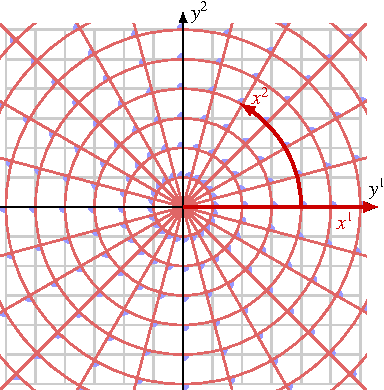
\includegraphics{papers/diffortho/images/polar.pdf}
\caption{Polarkoordinaten $(x^1,x^2)$ haben orthogonale Koordinatenlinien
({\color{darkred}rot})
und sind daher {\em orthogonale} Koordinaten.
\label{diffortho:fig:polar}}
\end{figure}
%
Die wohlbekannten Koordinatensysteme wie kartesische Koordinaten oder
Polarkoordinaten sind nicht beliebig.
Sie haben die zusätzliche Eigenschaft, dass die Koordinatenlinien
orthogonal sind, wie dies in Abbildung~\ref{diffortho:fig:polar}
am Beispiel der Polarkoordinaten gezeigt wird.
Es gilt daher zunächst, diese Eigenschaft zu charakterisieren.

\begin{definition}
Ein Koordinatensystem heisst {\em orthogonal}, wenn die Koordinatenlinien
orthogonal sind.
\index{orthogonale Koordinaten}%
\index{Koordinaten, orthogonal}%
\end{definition}

Seien 
\[
y^k
=
y^k(x^1,\dots,x^n)
\]
die Funktionen, die die Koordinatentransformation von den
$(x^1,\dots,x^n)$-Koordinaten in kartesische Koordinaten
$(y^1,\dots,y^n)$ transformiert.
Die $x^i$-Koordinatenlinien sind gegeben durch die Abbildungen
\[
t \mapsto y^k(x^1,\dots,\underset{\clap{$\uparrow\atop i$}}{t},\dots,x^n)
\]
gegeben.
Die Komponenten des Tangentialvektors an die $x^i$-Koordinatenlinie
an der Stelle $(x^1,\dots,x^n)$ sind durch die partiellen Ableitungen
\[
\xi^k
=
\frac{\partial y^k}{\partial x^i}
=
J^k\mathstrut_i
\]
nach $x^i$ gegeben.
Die Komponenten $\xi^k$ bilden die Spalte $i$ der Jacobi-Matrix
$J^k\mathstrut_i$.
\index{Jacobi-Matrix}%

Die Tangentialvektoren verschiedener Koordinatenlinien sollen orthogonal
sein.
Da die $y^i$-Koordinaten kartesisch sind, ist das Skalarprodukt zweier
Vektoren einfach die Summe der Produkte der Komponenten der beiden Vektoren.
Die Skalarprodukte der Tangentialvektoren an die Koordinatenlinien sind
auch bekannt als die Gram-Matrix dieser Basis, oder als der metrische
Tensor in diesem Koordinatensystem.
\index{Gram-Matrix}%
\index{metrischer Tensor}%
\index{Tensor, metrisch}%
Da die Vektorkomponenten die Spalten der Jacobi-Matrix sind, sind die
Einträge der Gram-Matrix die Skalarprodukte der Tangentialvektoren der
$x^i$- und der $x^j$-Koordinatenlinien
\[
g_{ij}(x)
=
\biggl(
\sum_{k=1}^n
\frac{\partial y^k}{\partial x^i}
\frac{\partial}{\partial x^k}
,
\sum_{l=1}^n
\frac{\partial y^l}{\partial x^j}
\frac{\partial}{\partial x^l}
\biggr)
=
\sum_{k=1}^n
\frac{\partial y^k}{\partial x^i}
\frac{\partial y^k}{\partial x^j}
=
\sum_{k=1}^n
J^k\mathstrut_i
J^k\mathstrut_j
=
(J^tJ)_{ij}.
\]
Die Tangentialvektoren für $i\ne j$ stehen senkrecht, wenn die
Skalarprodukte verschwinden.
Damit ist der folgende Satz gezeigt.

\begin{satz}
Die $y^k$-Koordinaten, die mit
\[
y^k
=
y^k(x^1,\dots,x^n)
\]
in kartesische Koordinaten umgerechnet werden können, sind genau dann
orthogonal, wenn die $J^tJ$ diagonal ist, wobei $J$ die Jacobi-Matrix
ist.
\end{satz}

In einem orthogonalen Koordinatensystem ist der metrische Tensor $g = J^tJ$
also diagonal und kann daher in der Form
\[
g
=
J^tJ
=
\begin{pmatrix}
 h_1(x)^2 &   0    & \dots  &    0   \\
   0    & h_2(x)^2 & \dots  &    0   \\[-2pt]
 \vdots & \vdots & \ddots & \vdots \\
   0    &   0    & \dots  & h_n(x)^2
\end{pmatrix}
\]
geschrieben werden.
Auf der Diagonalen steht die quadrierte Länge der Tangentialvektoren.
Die Diagonalelement $h_i(x)$ heissen auch die {\em metrischen Faktoren}
\index{Faktoren, metrisch}%
\index{metrische Faktoren}%
des orthogonalen Koordinatensystems.

\begin{beispiel}
Polarkoordinaten $(r,\varphi)=(x^1,x^2)$ werden durch die
\index{Polarkoordinaten}%
Transformationsgleichungen
\begin{equation*}
\renewcommand{\arraycolsep}{2pt}
\begin{array}{rclcl}
y^1 &=& r \cos\varphi &=& x^1 \cos x^2 \\
y^2 &=& r \sin\varphi &=& x^1 \sin x^2
\end{array}
\end{equation*}
Die Jacobi-Matrix ist
\[
J
=
\begin{pmatrix}
\cos x^2 &          - x^1 \sin x^2 \\
\sin x^2 & \phantom{-}x^1 \cos x^2
\end{pmatrix}.
\]
Das Produkt $J^tJ$ ist
\begin{align*}
J^tJ
&=
\begin{pmatrix}
\phantom{-x^1}\cos x^2 & \phantom{x^1}\sin x^2 \\
         -x^1 \sin x^2 &          x^1 \cos x^2
\end{pmatrix}
\begin{pmatrix}
\cos x^2 &          - x^1 \sin x^2 \\
\sin x^2 & \phantom{-}x^1 \cos x^2
\end{pmatrix}
\\
&=
\begin{pmatrix}
\cos^2 x^2 + \sin^2 x^2
&-x^1\cos x^2\sin x^2 + x^1\sin x^2\cos x^2
\\
-x^1\sin x^2\cos x^2 +x^1\cos x^2\sin x^2
&(x^1)^2 \sin^2 x^2 + (x^1)^2 \cos^2 x^2
\end{pmatrix}
\\
&=
\begin{pmatrix}
1 & 0 \\
0 & -(x^1)^2
\end{pmatrix}.
\end{align*}
Da dies eine Diagonalmatrix ist, sind Polarkoordinaten orthogonal.
\end{beispiel}

Die Tangentialvektoren an die Koordinatenlinien orthogonaler Koordinaten
sind orthogonal, aber haben nicht Einheitslänge.
Division durch $h_i(x)$ bringt sie auf Einheitslänge.
Sei der Vektor $g_i(x)$ gegeben durch die Komponenten
\[
\frac{1}{h_i(x)}
\frac{\partial y^k}{\partial x^i}
\]
mit $k=1,\dots,n$.
Dann sind die Vektoren $g_k(x)$ orthonormiert.

\begin{beispiel}
Kugelkoordinaten $(\vartheta,\varphi,r)$ sind durch die
\index{Kugelkoordinaten}%
Transformationsgleichungen
\begin{equation*}
\begin{array}{rcl}
y^1
&=&
r \sin\vartheta \cos\varphi
\\
y^2
&=&
r \sin\vartheta \sin\varphi
\\
y^3
&=&
r \cos\vartheta 
\end{array}
\end{equation*}
gegeben.
Die Jacobi-Matrix ist
\[
J
=
\begin{pmatrix}
r\cos\vartheta\cos\varphi
&-r\sin\vartheta\sin\varphi
&\sin\vartheta\cos\varphi
\\
r\cos\vartheta\cos\varphi
&r\sin\vartheta\cos\varphi
&\sin\vartheta\sin\varphi
\\
-r\sin\vartheta
&0
&\cos\vartheta
\end{pmatrix}.
\]
Das Produkt $J^tJ$ ist

\begin{align*}
J^tJ
&=
\renewcommand{\arraycolsep}{2pt}
\begin{pmatrix}
r\cos\vartheta\cos\varphi
&r\cos\vartheta\cos\varphi
&-r\sin\vartheta
\\
-r\sin\vartheta\sin\varphi
&r\sin\vartheta\cos\varphi
&0
\\
\sin\vartheta\cos\varphi
&\sin\vartheta\sin\varphi
&\cos\vartheta
\end{pmatrix}
\begin{pmatrix}
r\cos\vartheta\cos\varphi
&-r\sin\vartheta\sin\varphi
&\sin\vartheta\cos\varphi
\\
r\cos\vartheta\cos\varphi
&r\sin\vartheta\cos\varphi
&\sin\vartheta\sin\varphi
\\
-r\sin\vartheta
&0
&\cos\vartheta
\end{pmatrix}
\\
&=
%               [  2    2              2           2        2    2        ]
%               [ r  sin (theta) + (sin (phi) + cos (phi)) r  cos (theta) ]
%               [                                                         ]
%(%o7)  Col 1 = [                            0                            ]
%               [                                                         ]
%               [       2           2                                     ]
%               [   (sin (phi) + cos (phi) - 1) r cos(theta) sin(theta)   ]
%         [                   0                    ]
%         [                                        ]
% Col 2 = [     2           2        2    2        ]
%         [ (sin (phi) + cos (phi)) r  sin (theta) ]
%         [                                        ]
%         [                   0                    ]
%         [     2           2                                   ]
%         [ (sin (phi) + cos (phi) - 1) r cos(theta) sin(theta) ]
%         [                                                     ]
% Col 3 = [                          0                          ]
%         [                                                     ]
%         [      2           2          2             2         ]
%         [  (sin (phi) + cos (phi)) sin (theta) + cos (theta)  ]
\begin{pmatrix}
r^2\sin^2\vartheta + (\sin^2\varphi+\cos^2\varphi) r^2\cos^2\vartheta
& 0
& r(\sin^2\varphi+\cos^2\varphi-1)\cos\vartheta\sin\vartheta
\\
0
&\clap{$(\sin^2\varphi+\cos^2\varphi)r^2\sin^2\vartheta$}
&0
\\
(\sin^2\varphi+\cos^2\varphi -1)\cos\vartheta\sin\vartheta
&0
&(\sin^2\varphi+\cos^2\varphi)\sin^2\vartheta + \cos^2\vartheta
\end{pmatrix}
\\
%(%i8) trigsimp(P)
%                           [  2                    ]
%                           [ r         0         0 ]
%                           [                       ]
%(%o8)                      [      2    2           ]
%                           [ 0   r  sin (theta)  0 ]
%                           [                       ]
%                           [ 0         0         1 ]
&=
\begin{pmatrix}
r^2 &         0           & 0 \\
 0  & r^2 \sin^2\vartheta & 0 \\
 0  &         0           & 1
\end{pmatrix}.
\end{align*}
Somit sind auch Kugelkoordinaten orthogonal.
Die Vektoren $g_i(x)$ sind in diesem Fall
\[
g_1
=
\begin{pmatrix}
\cos\vartheta\cos\varphi\\
\cos\vartheta\sin\varphi\\
-\sin\vartheta
\end{pmatrix}
,\qquad
g_2
=
\begin{pmatrix}
\sin\varphi\\
\cos\varphi\\
0
\end{pmatrix}
\qquad\text{und}\qquad
g_3
=
\begin{pmatrix}
\sin\vartheta\cos\varphi\\
\sin\vartheta\sin\varphi\\
\cos\vartheta
\end{pmatrix},
\]
die sofort durch Nachrechnen als orthonormiert verifiziert werden können.
\end{beispiel}

Komplex differenzierbare Funktionen
$f\colon\mathbb{C}\to\mathbb{C}:z\mapsto f(z)$
stellen konform Abbildungen der komplexen Ebene dar.
Die durch
\[
y^1 + y^2i
=
f(x^1 + x^2i)
\]
definierte eine orthogonale Koordinatentransformation.
%
% fig-bipolar.tex
%
% (c) 2025 Prof Dr Andreas Müller
%
\begin{figure}
\centering
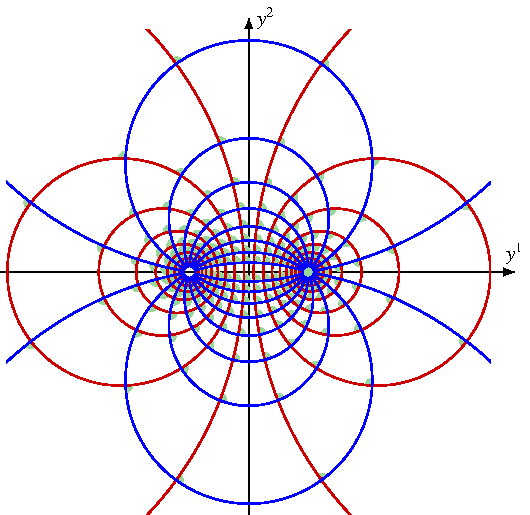
\includegraphics{papers/diffortho/images/bipolar.pdf}
\caption{Die Feldlinien und Äquipotentiallinien des Potentials
zweier Punktladungen in den Punkten $(\pm 1,0)$ können als Real-
und Imaginärteil der komplexen Funktion $y^1 + iy^2=\coth(x^1+ix^2)$ 
erzeugt werden.
Da komplexe Funktionen konforme Abbildungen der Ebene darstellen,
ist das $x^1$-$x^2$-Koordinatensystem orthogonal.
\label{diffortho:fig:bipolar}}
\end{figure}
%
Die Abbildung~\ref{diffortho:fig:bipolar} zeigt als Beispiel
die durch die meromorphe Funktion $f(z) = \coth(z)$ definiert
Abbildung.
Durch Einsetzen der Definition der hyperbolischen Cotangens-Funktion
und Anwendung der Additionstheoreme kann die reelle Schreibweise der
Funktion als
%(%i3) trigsimp(realpart(z))
%                   sinh(2 u) cos(2 v) + cosh(2 u) sinh(2 u)
%(%o3)              ----------------------------------------
%                               2            2
%                            sin (2 v) + sinh (2 u)
%(%i4) trigsimp(imagpart(z))
%                         (cos(2 v) + cosh(2 u)) sin(2 v)
%(%o4)                  - -------------------------------
%                                2            2
%                             sin (2 v) + sinh (2 u)
\begin{align*}
y^1
&=
\frac{
\sinh(2x^1)\cos(2x^2)+\cosh(2x^1)\sinh(2x^1)
}{
\sin^2(2x^2)+\sinh^2(2x^1)
}
\\
y^2
&=
-\frac{
(\cos(2x^2)+\cosh(2x^1))\sin(2x^2)
}{
\sin^2(2x^2)+\sinh^2(2x^1)
}
\end{align*}
gefunden werden.
Damit lassen sich die Koordinatenlinien als Linien mit einer
konstanten Koordinate zeichnen.
Sie können auch als die Feldlinien und Äquipotentiallinien des
elekrostatischen Feldes zweier Punktladungen in den Punkten $(\pm,0)$
der Ebene aufgefasst werden.



